% !TeX root = ../../main.tex
% Add the above to each chapter to make compiling the PDF easier in some editors.

\section{Generalization over domains}\label{ord:ch5:sec2}
% RE-1467

% Motivation - get insights of the performance on other domains (anomaly and industrial)
The ability of methods to generalize well may be crucial to their success in application.
For \gls{dl} methods the generalization capability is mostly based on the dataset used for training.
The \gls{iog} and \gls{dextr} method are trained on a combination of PASCAL \gls{voc} and COCO.
These datasets mostly cover general objects and do not contains images from special domains.
Therefore, the methods are evaluated on several image domains.
First, the generalization capabilities of the four benchmark methods are evaluated over image domains from the benchmark study.
Second, simulations are used to apply the \gls{iog} and \gls{dextr} methods on various datasets.

\subsection{Generalization over the Benchmark Domains}
% For all methods - Kruskal-Wallis test (or even ANOVA) for the domains as factors
The sample is split up by the benchmark domains, introduced in Section \ref{ord:ch4:sec4}, and evaluated for each domain.
For this the Kruskal-Wallis test is applied to each split with the four benchmark methods as factors.
Due to the split by the four domains and the requirement of the same factor size by the Kruskal-Wallis test, the number of samples per factor is reduced to $n_{annots}$ in this test setup.
The details and results of the tests is shown in Table \ref{tab:ch5:tests_on_domains} and the corresponding box plot of illustrated in Figure \ref{fig:ch5:sec2:domains_boxp_lot}.

For the domains $ Standard $ and $ Urban $, which are similar to PASCAL \gls{voc} and COCO, $ H_{0} $ is accepted and the benchmark methods do not differ significantly.
In contrast, for the domains $ Industrial $ and $ Anomaly $ $ H_{0} $ is rejected and $ H_{A} $ accepted. Therefore, there is some significant difference between the benchmark methods.
\begin{table}[h!]
	\centering
	\begin{tabular}{l|p{25mm} p{25mm} p{25mm} p{25mm}}
		\toprule 		
							& \centering $ Standard $	& $ Industrial $  & $ Anomaly $ & $ Urban $ \\
		\midrule
		$n_{annots}$		& 81			& 328 			  & 82			& 69 		\\
		$H_{0}$				& \multicolumn{4}{c}{$med \left( IoU_{polygon} \right) = med \left( IoU_{watershed} \right) = med \left( IoU_{IOG} \right) = med \left( IoU_{DEXTR} \right)$}  \\  
	%	$H_{0}$				& $med \left( IoU_{polygon} \right) =$ & $ med \left( IoU_{watershed} \right) =$ & $ med \left( IoU_{IOG} \right) =$ & $ med \left( IoU_{DEXTR} \right)$  \\		
		$H_{A}$		 		&  \multicolumn{4}{c}{$H_{0} = false$}  \\ 	
		$\alpha$		 	& $1\%$ 		& $1\%$ 		  & $1\%$ 		& $1\%$ 	\\ 	
		Statistic		 	& 2.9793		& 30.071	      & 15.4029		& 8.4354   	\\ 
		$\textnormal{\textit{p-value}}$
							& 0.3948		& $1.3 * 10^{-6}$ & 0.0015		& 0.0378	\\
		$H_{0}$		  		& accepted 		& rejected		  & rejected 	& accepted  \\ 										
		\bottomrule
	\end{tabular}
	\caption[Kruskal-Wallis tests over domains]{
		Four Kruskal-Wallis tests are applied for the domain scopes $ Standard $, $ Industrial $, $ Anomaly $, and $ Urban $.
		The four benchmark methods are used as factors for each test.
		For all tests the underlying sample is $X_{raw}$.
	}\label{tab:ch5:tests_on_domains}
\end{table}
%TODO allgin table properly

The post analysis is performed by the DSCF test \cite{CF91-dscf}, which determines the factor, that differs significantly in the domains $ Industrial $ and $ Anomaly $.
As a result, for the domain $ Industrial $ only the \gls{iog} method gave evidence for a statistical significant decrease in performance.
In the domain $ Anomaly $ two groups are formed, \gls{dextr} and Polygon achieve a significantly higher $ IoU $ than \gls{dextr} and Watershed.
Inside these two groups no significant difference occurs.
% Box plot with 16 "cols" - 4 methods x 4 domains
\begin{figure}
	\centering
	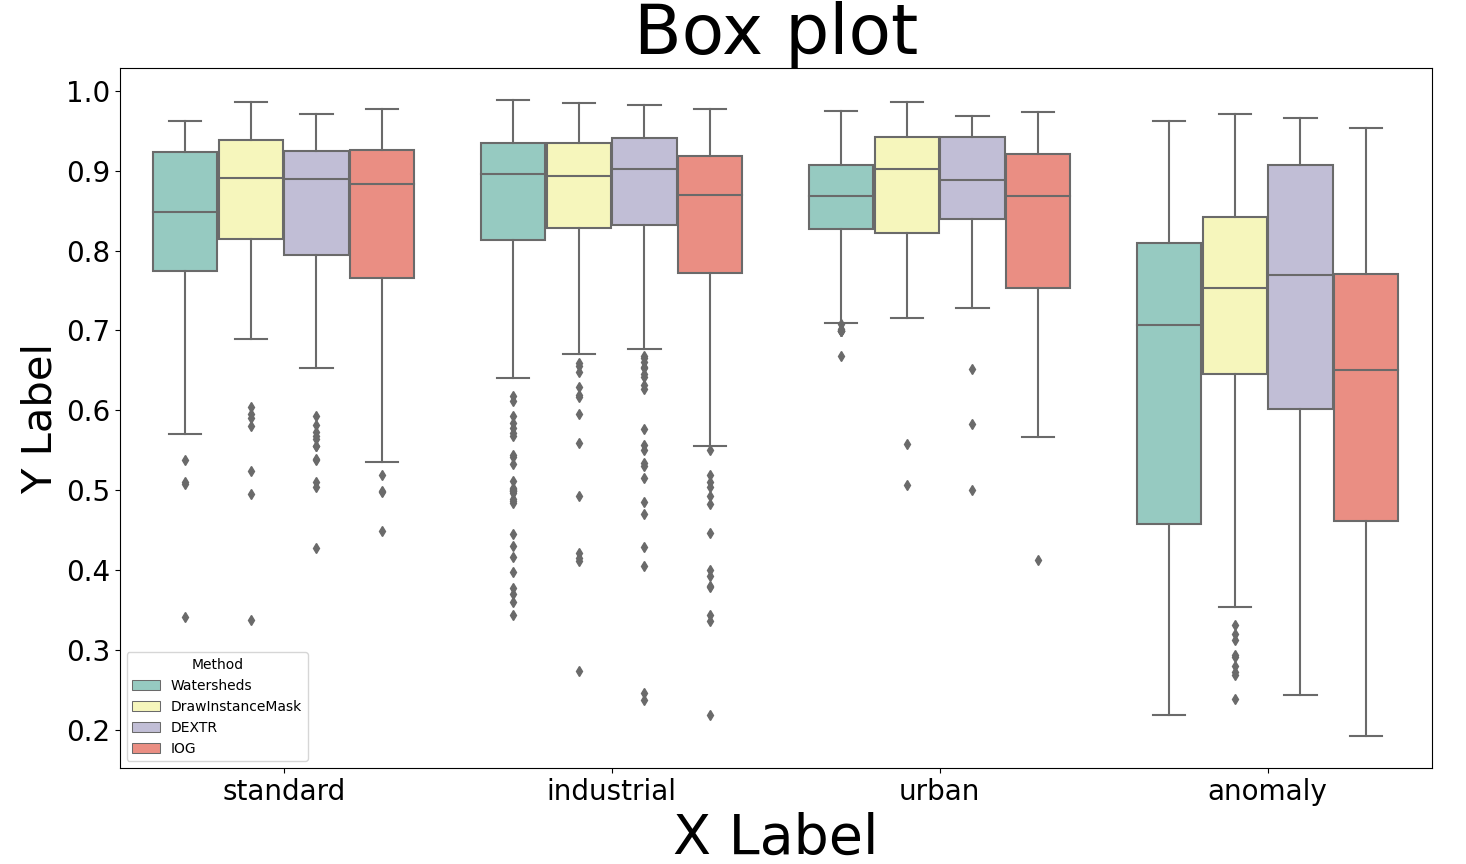
\includegraphics[width=0.9\textwidth]{figures/chap52_boxplot.png}
	\caption[Box plot IoU per domain and method]{
		Box plot of the $IoU$ per image domain and benchmark method.
	} \label{fig:ch5:sec2:domains_box_plot}
\end{figure}

Further, it was detected, that the domains $ Standard $, $ Industrial $, and $ Anomaly $ do not differ significantly in their median value of the $IoU$.
Only the domain scope $ Anomaly $ differs greatly, which is reasonable due to the clearly different types of images.
It was experienced in the review of the user annotations, that the users often have a varying understanding what belongs to the anomaly, which should be labeled.
This ranges from different to misinterpretations, which also in an explanation for the general lower $ IoU $ in this domain.
The good performance of the polygon and \gls{dextr} method in the domain $ Anomaly $ most probably is caused by the strong and direct type of guidance provided by the user interaction.

In conclusion it may be stated, that the examined benchmark methods mostly do not significantly vary over common domains, excluding the domain $ Anomaly $.
Only for the \gls{iog} method did not generalize as well as the other methods on the domain $ Industrial $.


\subsection{Generalization over different Datasets}

In order to further evaluate the \gls{dextr} and \gls{iog} method, simulations are applied on various datasets.
To continue the evaluation of the generalization capabilities datasets from different domains are used.
First, the performance of the initial prediction is presented, while later the refinement results are examined. 

\subsubsection{Initial Prediction}

% Define simulation settings
The different simulation setups from the original \gls{dextr} \cite{Man18-DEXTR} and \gls{iog} \cite{Zha20-IOG} have been implemented in HDevelop and unified to allow a fair comparison. 
Thereby, the \gls{gt} is used to simulate the user clicks on fore- and background to create the required model input.
It has to be highlighted, that this simulation setup only contains little deviation or randomness, similar to the original simulation setup from \gls{dextr} and \gls{iog}.
As a result, the simulated user clicks are almost perfect.
More realistic user clicks can be simulated by the inclusion of random deviation, which is presented in Section \ref{ord:ch5:sec3}.

The performance of the \gls{dextr} and \gls{iog} method on various datasets is shwon in Table \ref{tab:ch5:tests_on_datasets}.
As the output of the segmentation model is a probability map with, which predicts if a pixel either belongs to the foreground or background, a threshold needs to be applied.
The \gls{dextr} method performs best at a threshold of $ 0.5 $, while the best threshold value for \gls{iog} is $ 0.8 $.
The \gls{miou} values presented are achieved by the most suitable threshold value for each method.

It can be seen, that the examined methods perform very similar on the applied datasets.
This is interesting, because the \gls{dextr} method gave the impression to be advantageous in the previous evaluation.
% TODO Vermutung, dass die DEXTR methode intiuitiver ist und für echte User bessere ergebnisse Einfährt als IOG

%TODO apply more datasets?
\begin{table}[h!]
	\centering
	\begin{tabular}{l|c c}
		\toprule 		
									& \gls{miou} by \gls{dextr} &\gls{miou} by \gls{iog}	\\
		% Threshold					& 0.5 	& 0.8 		& 0.5  		& 0.8 		\\
		\midrule
		PASCAL VOC (VP \cmark)	& 0.9103 	& 0.9251	\\
		PASCAL VOC (VP \xmark)	& 0.7805	& 0.8086	\\
		Benchmark Dataset			& 0.8394 	& 0.8201	\\
		D2S							& 0.9297	& 0.9342	\\
		MAD	??						& - 	& -		\\
		Segmentation and Counting??	& -		& - 	\\
		tbd	??						& -		& - 	\\
		% PASCAL VOC 2012	VP \cmark	& -		& 0.9103 	& 0.9251	& 0.8945	\\
		% PASCAL VOC 2012 VP \xmark	& -		& 0.7805	& 0.8086	& 0.8195	\\
	    % Benchmark Dataset			& 0.8380	& 0.8394 	& 0.8201	& 0.7787	\\
		% D2S							& -		& 0.9297	& 0.9342	& 0.9158	\\
		% MAD	??						& -		& - 	& -		& -		\\
		% Segmentation and Counting ??	& -		& - 	& -		& -		\\
		% tbd	??						& -		& - 	& -		& -		\\											
		\bottomrule
	\end{tabular}
	\caption[Generalization of IOG and DEXTR]{
		The \gls{dextr} and \gls{iog} method are applied on multiple datasets to evaluate their performance over several domains.
		The performance is measured by the \gls{miou}.
		VP \cmark and VP \xmark \space represent the evaluation with and without the use of the void pixel.
	}\label{tab:ch5:tests_on_datasets}
\end{table}

% point out weakness of void pixel
The dubious use of void pixel already is pointed out in the introduction of the PASCAL \gls{voc} dataset \cite{Eve20-PascalVOC} from Subsection \ref{ord:ch2:sec2}.
The effect of void pixel on the \gls{miou} can be seen clearly, the difference is up to almost 13\%.
By the presentation of such results, unrealistic expectations are raised on the method's performance, which are mostly not achievable in real world application.

\subsubsection{Refinement Prediction}

% Show a table displaying the performance for various refinement clicks on multiple dataset
Last, the performance of the method with the application of refinement is evaluated on different datasets.
Thereby, for each method five refinement clicks were simulated.
For the \gls{iog} method, the refinement clicks can be on the fore-and background, while the \gls{dextr} methods only allows refinement clicks on the border, which are categorized as foreground clicks.
The refinement clicks are simulated using the \gls{gt}.
A click is set on the greatest error region from the previous prediction.

In Table \ref{tab:ch5:tests_on_refinement datasets} the performance of the methods is presented for various refinement clicks.
For \gls{dextr} mostly only the first refinement clicks leads to a improvement, while the further clicks keep or decrease the \gls{miou}.
In contrast, the \gls{iog} method is able to profit from each refinement click and increase the \gls{miou}. 
From the ninth click, the improvement stagnates or worsens slightly as shown in Appendix XXX. 
% TODO ref appendix and add simulation with 20 refinement clicks.  
It can be stated, that refinement process generalizes well and performs expected over several domains.

\begin{table}[h!]
	\centering
	\begin{tabular}{l l|c c c c c c}
		\toprule
				&						& \multicolumn{6}{c}{\gls{miou} for $ n_{\textnormal{\textit{refine clicks}}} $ refinement clicks } \\
				& {$ n_{\textnormal{\textit{refine clicks}}} $} 
										& 0			& 1			& 2			& 3 		& 4 		& 5			\\
		\midrule
		DEXTR 	& PASCAL VOC (VP \cmark)	& 0.9103	& 0.9119	& 0.9054	& 0.8986 	& 0.8916	& 0.8863	\\
			 	& PASCAL VOC (VP \xmark)	& 0.7805	& 0.7894 	& 0.7893	& 0.7871 	& 0.7833	& 0.7807	\\
				& Benchmark Dataset		& 0.8394	& 0.8522 	& 0.8513	& 0.8504 	& 0.8512	& 0.8492	\\
				& D2S					& 0.9297	& 0.9416 	& 0.9436	& 0.9437 	& 0.9419	& 0.9397	\\
		\midrule
		IOG 	& PASCAL VOC (VP \cmark)	& 0.9251	& 0.9359	& 0.9402	& 0.9436 	& 0.9449	& 0.9459	\\
				& PASCAL VOC (VP \xmark)	& 0.8086	& 0.8184	& 0.8259	& 0.8313 	& 0.8351	& 0.8381	\\
				& Benchmark Dataset		& 0.7843	& 0.7992 	& 0.8075	& 0.8146 	& 0.8191	& 0.8219	\\
				& D2S					& -		& - 	& -		& - 	& -		& -		\\
		\bottomrule
	\end{tabular}
	\caption[Generalization of IOG and DEXTR Refinement]{
		Performance of the \gls{dextr} and \gls{iog} method for various refinement clicks.
		At $ n_{\textnormal{\textit{refine clicks}}} = 0 $, no refinement click is set, which is equivalent to the initial prediction.
	}\label{tab:ch5:tests_on_refinement datasets}
\end{table}
